\documentclass[border=10pt]{standalone}
\usepackage{pgfplots}
\pgfplotsset{width=10cm,compat=1.8}
\begin{document}
\begin{tabular}{c}
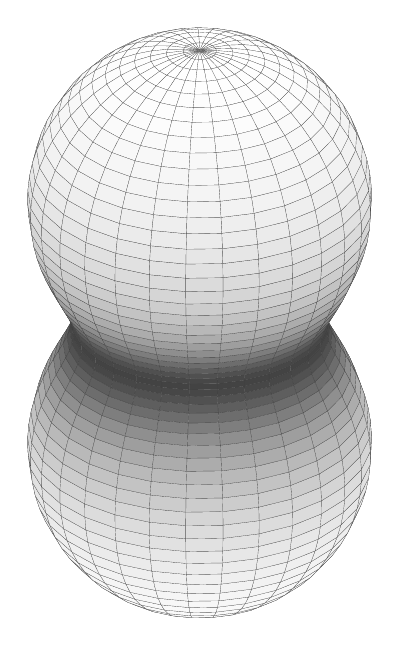
\begin{tikzpicture}
  \begin{axis}[
    hide axis,
    clip=false,
    y domain=0:180,
    samples=30,
    axis equal,
    view={45}{30},
    width=25cm,
    at={(0cm,0cm)},
    %colorbar,
    %colorbar/width=1cm,
    %colorbar horizontal,
    %colorbar style={
    %  height=1cm,
    %  yshift=-0.4cm,
    %  ytick={-1,1}
    %},
    colormap={iron}{[1pt]rgb255(-1000pt)=(255,255,255),rgb255(-998pt)=(255,255,255),rgb255(-991pt)=(255,255,255),rgb255(-980pt)=(254,254,254),rgb255(-964pt)=(254,254,254),rgb255(-944pt)=(253,253,253),rgb255(-920pt)=(252,252,252),rgb255(-892pt)=(251,251,251),rgb255(-861pt)=(250,250,250),rgb255(-826pt)=(249,249,249),rgb255(-789pt)=(247,247,247),rgb255(-749pt)=(245,245,245),rgb255(-707pt)=(243,243,243),rgb255(-664pt)=(240,240,240),rgb255(-619pt)=(237,237,237),rgb255(-573pt)=(233,233,233),rgb255(-527pt)=(228,228,228),rgb255(-480pt)=(223,223,223),rgb255(-435pt)=(217,217,217),rgb255(-390pt)=(210,210,210),rgb255(-346pt)=(202,202,202),rgb255(-304pt)=(193,193,193),rgb255(-264pt)=(183,183,183),rgb255(-226pt)=(171,171,171),rgb255(-190pt)=(157,157,157),rgb255(-158pt)=(143,143,143),rgb255(-127pt)=(127,127,127),rgb255(-100pt)=(111,111,111),rgb255(-74pt)=(96,96,96),rgb255(-51pt)=(83,83,83),rgb255(-29pt)=(73,73,73),rgb255(-8pt)=(67,67,67),rgb255(12pt)=(68,68,68),rgb255(33pt)=(75,75,75),rgb255(55pt)=(85,85,85),rgb255(78pt)=(99,99,99),rgb255(104pt)=(114,114,114),rgb255(132pt)=(130,130,130),rgb255(163pt)=(145,145,145),rgb255(196pt)=(160,160,160),rgb255(232pt)=(173,173,173),rgb255(270pt)=(184,184,184),rgb255(311pt)=(195,195,195),rgb255(353pt)=(204,204,204),rgb255(397pt)=(212,212,212),rgb255(442pt)=(218,218,218),rgb255(488pt)=(224,224,224),rgb255(534pt)=(229,229,229),rgb255(581pt)=(233,233,233),rgb255(626pt)=(237,237,237),rgb255(671pt)=(240,240,240),rgb255(714pt)=(243,243,243),rgb255(756pt)=(245,245,245),rgb255(796pt)=(247,247,247),rgb255(832pt)=(249,249,249),rgb255(866pt)=(250,250,250),rgb255(897pt)=(252,252,252),rgb255(924pt)=(253,253,253),rgb255(948pt)=(253,253,253),rgb255(967pt)=(254,254,254),rgb255(982pt)=(254,254,254),rgb255(992pt)=(255,255,255),rgb255(998pt)=(255,255,255)}
    ]

  \addplot3 [
      domain=0:360,
      surf,
      shader=flat,
      z buffer=sort,
      %fill=white!50!gray,
      draw=gray!50!black,
      line join=bevel,
      line width=0.002cm,
      samples y=60
    ]
    ( {sqrt(0.2+cos(y)^2)*sin(y)*cos(x)},
      {sqrt(0.2+cos(y)^2)*sin(y)*sin(x)},
      {sqrt(0.2+cos(y)^2)*cos(y)}
    );
    -- cycle;
   \end{axis}
\end{tikzpicture}
\\
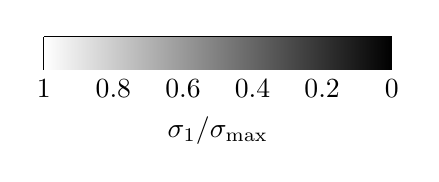
\begin{tikzpicture}
  %A-opt countour
\begin{axis}[%
view={0}{90},
shader=interp,
%3d box=complete,
grid=major,
xlabel = {$\sigma_1/\sigma_{\mathrm{max}}$},
xmin = 0, xmax = 1,
ymin = 0, ymax =1,
view/h=-180,
width=6cm,
height=2cm,
at={(9.5cm,4cm)},
    colormap={blackwhite}{[1cm] rgb255(0cm)=(0,0,0) rgb255(1cm)=(255,255,255)},
yticklabels={,,}
],

\addplot3[%
surf,
samples=30,
domain=0:1,
y domain=0:1,
]
{x};
\end{axis}
\end{tikzpicture}
\end{tabular}
\end{document}